\chapter{Isotope-Dependent Optical Trapping}

This project ended up being a bit of a technical exploration trying to see if we could design a trap where we could tailor the trapping potential experienced by different isotopes when working with isotopic mixtures.
In particular, we sought to exploit the large isotope shift of the $\nSLJ{5s^2}{1}{S}{0} \rightarrow \nSLJ{5s5p}{3}{P}{1}$ transition ($\flatfrac{\Delta_{\text{isotope}}}{2 \pi} \sim \SI{100}{\MHz}$) compared to its linewidth ($\flatfrac{\Gamma_{\SI{689}{\nm}}}{2 \pi}=\SI{7.5}{\kHz}$).
Considering that $U_{\text{dip}} \sim \flatfrac{1}{\Delta}$ and $\Gamma_{\text{sc}} \sim \flatfrac{1}{\Delta^2}$ \cite{Grimm1999.arXiv.9902072}, it should be possible to produce an attractive potential for one isotope which is repulsive for another isotope. 
Using two lasers would allow us to provide a deep potential for one isotope whereas the potential is canceled for another isotope so that it experiences no additional trapping nor anti-trapping effects. 

\section{Challenges in Producing Quantum Degenerate Gases of \Sr{88} and \Sr{87}}

Although there have been recent developments towards producing quantum degenerate gases without evaporative cooling \cite{Stellmer2013.PRL.110.263003, Hu2017.Science.358.1078}, the methods presented have restrictive constraints. 
\citeauthor{Stellmer2013.PRL.110.263003} took advantage of the narrow $\nSLJ{5s^2}{1}{S}{0} \rightarrow \nSLJ{5s5p}{3}{P}{1}$ in \Sr{84} to maintain a cold reservoir of laser-cooled atoms which are collected in a dimple shielded by a ‘‘transparency'' but still requires elastic collisions for thermalization in the dimple.
\citeauthor{Hu2017.Science.358.1078} requires a two-dimensional optical lattice to perform cycles of Raman sideband cooling and compression in a gas of \Rb{87}.

One of the most interesting isotopes for studying quantum gases is \Sr{88} due to is high natural abundance and near-zero \Sr{88}-\Sr{88} $s$-wave scattering length (see see \cref{tab:sr_scattering_lengths_long}), making it an ideal candidate for studying non-interacting BECs.
Early work towards producing quantum degenerate gases of strontium focused on \Sr{88} \cite{Ido2000.PRA.61.061403} and \Sr{88}-\Sr{86} mixtures \cite{Poli2005.PRA.71.061403} but the tight optical traps used hindered evaporation to quantum degeneracy due to \Sr{86}'s the large three-body recombination rate \cite{Ferrari2006.PRA.73.023408}.
Currently, the only method for demonstrated for producing \Sr{88} BECs requires sympathetic cooling with either \Sr{87} \cite{Mickelson2010.PRA.81.051601, Stellmer2013.PRA.87.013611} or \Sr{86} \cite{Stellmer2013.PRA.87.013611}.
Neglecting the added complexity of narrow line cooling \Sr{87}, sympathetic cooling \Sr{88} with \Sr{87} has been shown to be promising with relative quick evaporations with properly tailored traps \cite{Stellmer2013.PRA.87.013611} but is potentially slowed by the modest $a_{88,87} \approx \SI{55}{\bohr}$ and Pauli blocking of collisions between \Sr{87} atoms which leads to inefficient evaporation once the fermions becomes quantum degenerate \cite{DeSalvo2010.PRL.105.030402}.
Sympathetic cooling \Sr{88} with \Sr{86} would be ideal due to the large natural abundances of both isotopes, the simplified narrow line cooling laser system required, and the convenient $a_{88,86} \approx \SI{97}{\bohr}$ but, as noted above, \Sr{86} requires a large-volume trap to mitigate three-body loses. 

Being able to quickly produce \Sr{88} BECs are nearly ``perfect'' non-interacting Bosons with no nuclear spin. 
Considering that \Sr{88} BECs are typically very small (** ADD REFERENCE AND/OR CALCULATION **) due to the slightly negative {$s$-wave} scattering length, there's interest in studying how the Rydberg electron couples to a BEC \cite{Balewski2013.Nature.12592} and, as $n$ increase, ion-BEC interactions \cite{Kleinbach2018.PRL.120.193401} without needing electrodes for an ion trap.
The small \Sr{88} BEC is almost non-interacting also makes it a great candidate for observing three-dimensional solitons \cite{Maucher2011.PRL.106.170401} as it should be easier to Rydberg dress the entire BEC and there's less mean field interaction energy.

There's also interest in degenerate Fermi gases (DFG) of \Sr{87} due to its large nuclear spin ($I=\flatfrac{9}{2}$) for qubit registers \cite{Gorshkov2009.PRL.102.110503} and quantum simulation/{$SU\left(N\right)$} magnetism \cite{Gorshkov2010.NPhys.1535, Hazzard2012.PRA.85.041604, Pagano2014.NPhys.2878, Hofrichter2016.PRX.6.021030, Ozawa2018.PRL.121.225303} (** CHECK SOURCES/READ A FEW OF THEM **).

\section{Isotope-Dependent Optical Trapping}



***********************************

As previously mentioned, making \Sr{88} BECs requires sympathetic cooling (** ADD SOURCES **) due to $a_{88-88}=\SI{-2(1)}{\bohr}$. 
Making an \Sr{87} DFG is possible due to its ten spin states \cite{DeSalvo2010.PRL.105.030402} but producing a spin-polarized DFG also requires sympathetic cooling as identical fermions no longer collide \cite{Stellmer2013.PRA.87.013611} (** PROBABLY INCLUDE OTHER SOURCES AS WELL **).
Although having abysmal abundance, \Sr{84} has a nice {$s$-wave} scattering length of $a_{84-84}=\SI{122.762(92)}{\bohr}$ and is generally quite easy to make \Sr{84} BECs using the magnetic trap to capture enough atoms.

It's here that we note \Sr{86} has relatively nice {$s$-wave} scattering lengths with \Sr{88} ($a_{88-86}=\SI{97.374(69)}{\bohr}$) and \Sr{87} ($a_{87-86}=\SI{162.25(21)}{\bohr}$).
Coupled with it's plentiful abundance, \Sr{86} looks to be an ideal cooling for sympathetic cooling if the challenges of the large $a_{86-86}=\SI{798(12)}{\bohr}$ can be overcome.

Since the potential scales as $\flatfrac{\Gamma}{\Delta}$ whereas the off-resonant scattering scales as $\left(\flatfrac{\Gamma}{\Delta}\right)^2$, the idea here is to take advantage of the large isotope shift of the $\nSLJ{5s^2}{1}{S}{0} \rightarrow \nSLJ{5s5p}{3}{P}{1}$ ($\Delta \sim \SI{100}{\MHz}$) compared to the transition linewidth $\flatfrac{\Gamma}{2\pi} = \SI{7.5}{\kHz}$.

\subsection{Trap Design}

The trap geometry influences how evaporative cooling proceeds due to the density dependences of the elastic and inelastic collision rates. 
Based on the trapping geometries presented in \cite{Stellmer2013.PRA.87.013611}, we decided to use the large-volume $\SI{1064}{\nm}$ sheet trap to support the atoms against gravity and a nearly-vertical $\SI{689}{\nm}$ beam with a circular waist of about $\SI{60}{\um}$ to provide transverse confinement. 


***********************************

In order to form BECs of \Sr{86}, evaporative was performed at low density in a large-volume trap \cite{Stellmer2010.82.041602, Stellmer2013.PRA.87.013611}.
On the other hand, \Sr{88} BECs were achieved through sympathetic cooling with \Sr{87} in a tight trapping geometry. 
Therefore, we want the different isotopes to experience different confining potentials:
-\Sr{86} only experiences a large-volume trap.
-\Sr{88} and \Sr{87} experiences a tight-confining potential.

\begin{figure}[h]
	\centering
	\includesvg[keepaspectratio, width=4in, height=\textheight]{magic_trap/dimple_setup/dimple_and_sheet_geometry.svg}
	\caption{
		\label{fig:sheet_and_dimple_geometry}
		Geometry of the large-volume \SI{1064}{\nm} horizontal ``sheet'' trap and the tight vertical \SI{689}{\nm} ``dimple''.}
\end{figure}

The magic dimple would only provide transverse confinement with the sample temperature predominately set by the vertical trap depth of the horizontal \SI{1064}{\nm} sheet trap. 

The ``trap'' beam is generated by a GHz AOM used to injection lock the \Sr{87} trap slave. 
The ``cancel'' beam is generated from a slave injection locked closer to resonance. 

*** Add more details? ***
Based on our experiences with $\SI{60}{\um} \times \SI{60}{\um}$ crossed-beam \SI{1064}{\nm} ODT and the designs of other groups \cite{Stellmer2013.PRA.87.013611}, we decided to try starting with a $\SI{60}{\um} \times \SI{60}{\um}$ circular dimple propagating nearly vertically.
This waist size is relatively easy to generate with reasonably focal length lenses allowing us to place the setup somewhere convenient. 
\begin{figure}[h]
	\centering
	\includesvg[keepaspectratio, width=4in, height=\textheight]{magic_trap/dimple_setup/dimple_profile.svg}
	\caption{
		\label{fig:magic_dimple_profile}
		The dimple is relatively well described by a nearly-circular Gaussian beam with waists $w_{0,x}=\SI{64.9+-1.6}{\um}$ and $w_{0,y}=\SI{59.5+-1.1}{\um}$ located at $z_{0,x}=\SI{27.17+-0.07}{\cm}$ and $z_{0,y}=\SI{26.98+-0.07}{\cm}$.}
\end{figure}

The ``trap'' light is generated from RS3 injection locked at \SI{-1323.44}{\MHz} from the $\nSLJ{5s^2}{1}{S}{0} \rightarrow \nSLJ{5s5p}{3}{P}{1}$ in \Sr{88}, putting it about \SI{-82}{\MHz} detuned of the $\nSLJf{5s^2}{1}{S}{0}{9/2} \rightarrow \nSLJf{5s5p}{3}{P}{1}{11/2}$ transition needed for the operating an \Sr{87} red MOT. 
Since we needed an additional AOM to provide the amplitude modulation for lock-in power control, an additional \SI{-85}{\MHz} was applied, placing the final detuning of the ``trap'' beam at \SI{-1408.44}{\MHz}. 
The ``cancel'' light is generated from RS1 or RS2, both of which are injection locked at \SI{-82}{\MHz} and further shifted by AOMs at \SI{+110}{\MHz} and \SI{-120}{\MHz} to a final detuning around \SI{-92}{\MHz} (** Did we purposefully slightly bias it to be closer to \Sr{86} resonance instead of directly in between? **).
Although I didn't notice significant losses the frequencies for both the ``trap'' and ``cancel'' beams can be chosen to avoid photoassociation lines \cite{Zelevinsky2006.PRL.96.203201, Borkowski2014.PRA.90.032713, Reschovsky2018.arXiv.1808.06507}.

Now the beam size and ``trap'' and ``cancel'' frequencies are chosen, we can calculate the expected trap depths based on the power of each beam.

\subsection{Polarizability}

Working in the two-level approximation and considering only the $\ket{g} = \nSLJ{5s^2}{1}{S}{0}$ and $\ket{e} = \nSLJ{5s5p}{3}{P}{1}$ states, the AC dipole polarizability can be calculated as \cref{eq:ac_pol}
\begin{equation}
	\alpha	= \frac{2 \mel{g}{\va{d}}{e}^{2}}{\hbar}\frac{\omega_{0}}{\omega_{0}^{2} - \omega_{L}^{2}}
			= 6 \pi \epsilon_{0} c^{3} \Gamma \frac{1}{\omega_{0}^{2} \qty(\omega_{0}^{2} - \omega_{L}^{2})}
\end{equation}
and the potential is \cref{eq:U_odt} *** CHECK EQUATIONS ***
\begin{equation}
	U	= -\frac{3 \pi c^{2} \Gamma}{\omega_{0}^{2} \qty(\omega_{0}^{2} - \omega_{L}^{2})}
\end{equation}
** FIG. XXX ** shows the potential experienced by the (bosonic) isotopes


********************************************

********************************************

********************************************


** I'm not sure where I should put this section. **

** Talk about polarizability calculation here ! I still need to work through the derivation... **

Assuming that the AC Stark shift is dominated by the \SI{689}{\nm} transition, we make the two-level approximation where the potential experimenced by the atoms can be approximated by \cite{Grimm1999.arXiv.9902072}
\begin{align}
	U\qty(\vb{r})		&{}={}	-\frac{3 \pi c^2}{2 \omega_{0}^{3}} \qty(\frac{\Gamma}{\omega_{0}-\omega} + \frac{\Gamma}{\omega_{0}+\omega}) I\qty(\vb{r})	\\
	\Gamma\qty(\vb{r})	&{}={}	\frac{3 \pi c^2}{2 \hbar \omega_{0}^{3}} \qty(\frac{\omega}{\omega_{0}})^{2} \qty(\frac{\Gamma}{\omega_{0}-\omega} ++ \frac{\Gamma}{\omega_{0} + \omega})^{2} I\qty(\vb{r})
\end{align}
where $U\qty(\vb{r})$ is the potential and $\Gamma\qty(\vb{r})$ is the scattering rate (see appendix xxx for details... ** I still need to work through the derivation... **).

** Include note about the ``real'' polarizability accounting for other states (i.e., not in the two-level approximation)? See \cite{Boyd2007.PhD} **

\subsubsection{Lock-In Power Control}

\begin{figure}[h]
	\centering
	\includesvg[keepaspectratio, width=\textwidth, height=\textheight]{magic_trap/dimple_setup/dimple_power_control.svg}
	\caption{
		\label{fig:dimple_setup}
		Setup of the \SI{689}{\nm} dimple showing how the ``trap'' and ``cancel'' beams were chopped to facilitate lock-in power control.}
\end{figure}

Due to the requirements of having both the trap and cancel beams be perfectly mode-matched with the same polarizations, we decided to use lock-in detection to actively stabilize power of the two beams. 
This was accomplished by chopping the trap and cancel beams at two different frequencies, \SI{\sim500}{\kHz} and \SI{\sim200}{\kHz}, both significantly higher than the trap frequencies of the \SI{1064}{\nm} ODT and the predicted trap frequencies of the dimple.

\section{Single-Isotope Testing with \Sr{84}}

With some concerns of heating due to off-resonant scattering of the \SI{689}{\nm} ``trap'' and ``cancel'' beams, we first tested the dimple with just the ``trap'' beam (still being chopped at \SI{500}{\kHz}) in order to see how well we're able to evaporate with the dimple on.
We decided to work with \Sr{84} because it's easy to evaporate to quantum degeneracy.
\Cref{fig:dimple-84Sr_lifetime} shows that, at low powers, we don't observe much atom loss when just the \SI{689}{\nm} trap beam is applied.
\begin{figure}[h]
	\centering
	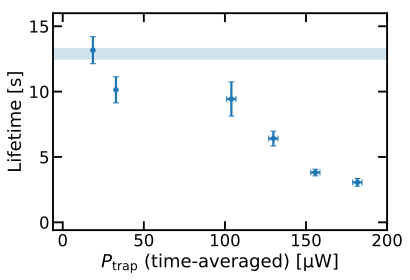
\includegraphics[keepaspectratio, width=4in, height=\textheight]{magic_trap/dimple_84Sr/dimple-84Sr_lifetime.pdf}
	\caption{
		\label{fig:dimple-84Sr_lifetime}
		Lifetime of \Sr{84} atoms in just the dimple region varying the (time-averaged) $P_\text{trap}$ (no cancel beam was applied). 
		The trap beam was detuned by $\flatfrac{\Delta_{\text{trap}}}{2\pi} = \SI{-886.51}{\MHz}$ from $\SLJ{1}{S}{0} \rightarrow \SLJ{3}{P}{1}$ resonance in \Sr{84} and chopped at $\SI{500}{\kHz}$ with a $\SI{50}{\percent}$ duty cycle.
		Horizontal shaded region represents the lifetime of atoms in just the sheet trap without the $\SI{689}{\nm}$ dimple.}
\end{figure}

With the promising result that the trap beam isn't causing significant atom loss we proceeded to try evaporating the sheet trap and compare with and without the dimple. 

******************************

The \SI{1064}{\nm} sheet trap provides tight confinement along gravity but loose confinement transversely. 
With xxx power in the ``trap'' beam, the transverse trap depth should be able to increase the transverse confinement to about xxx nK. 

In this configuration, we were able to produce an \Sr{84} BEC in just the sheet trap as well as in the dimple following the same intensity ramp of the sheet. 
(** Show images of evaporation in just sheet vs. evaporation in sheet + dimple **)

\subsection{Producing an \Sr{84} BEC in the Dimple}

\begin{figure}[h]
	\centering
	\includegraphics[keepaspectratio, width=\textwidth, height=\textheight]{magic_trap/dimple_84Sr/dimple_84Sr_BEC/drop_after_evaporation/sheet_dimple_comparison-drop.pdf}
	\caption{
		\label{fig:sheet_dimple_comparison-drop}
		Production of an \Sr{84} BEC with and without the dimple in the sheet trap.
		Absorption image taken after a \SI{40}{\ms} time-of-flight.}
\end{figure}

\begin{figure}[h]
	\centering
	\includesvg[keepaspectratio, width=\textwidth, height=\textheight]{magic_trap/dimple_84Sr/dimple_84Sr_results.svg}
	\caption{
		\label{fig:dimple_84Sr_results}
		Results of evaporating the sheet trap with and without the \SI{689}{\nm} dimple.}
\end{figure}

\section{Sympathetically Cooling \Sr{88} with \Sr{86}}

Sympathetically cooling of \Sr{88} with \Sr{86} was first reported by \citeauthor{Poli2005.PRA.71.061403} but they had difficulty reaching quantum degeneracy.

\begin{figure}[h]
	\centering
	\includesvg[keepaspectratio, width=\textwidth, height=\textheight]{magic_trap/dimple_88Sr-86Sr/dimple_88Sr-86Sr_results.svg}
	\caption{
		\label{fig:dimple_88Sr-86Sr_results}
		Results varying the evaporation time while maintaining the same final sheet trap depth (** CHECK!! **).}
\end{figure}

Possible observation of double-degeneracy with BECs of \Sr{88} and \Sr{86}. 

\begin{figure}[h]
	\centering
	\includesvg[keepaspectratio, width=\textwidth, height=\textheight]{magic_trap/dimple_88Sr-86Sr/possible_88Sr_86Sr_BECs.svg}
	\caption{
		\label{fig:possible_88Sr_86Sr_BECs}
		Possible observation of double-degeneracy of \Sr{88} and \Sr{86} forming BECs.
		Imaged after \SI{40}{\ms} drops and averaging 20 images.
		\Sr{86} is possibly not a BEC but expanding due to hydrodynmaics (** ASK TOM **).
		Our imaging system didn't have good enough resolution to confirm without further investigations.
		(** CHECK!! **)When imaging \Sr{88}, \Sr{86} was removed with a resonant \SI{689}{\nm} beam before imaging and vice-versa for imaging \Sr{86} to remove background atoms.}
\end{figure}

\section{Proposal Sympathetically Cooling \Sr{87} with \Sr{86}}

Using circularly polarized dimple beams should suppress off-resonant scattering off the intermediate state by coupling F=9/2 to F=11/2 in a spin-polarized gas.  

Somewhat similar have been previously proposed for trapping spin-polarized \Rb{85} \cite{Corwin1999.PRL.83.1311, Corwin1999.PhD} (** CHECCK !!**) or producing a spin-dependent optical lattice \cite{Mandel2003.PRL.91.010407, McKay2010.NJP.12.055013, Gadway2010.PRL.105.045303, Reimann2009.MA, Pertot2011.PhD, Gadway2012.PhD} (** CHECK!! **)

\section{Preliminary Conclusions and Future Directions}

We don't currently have the capability to conclusively determine whether a doubly-degenerate BEC was formed. Blah, blah, blah.

Along similar lines to previous work in rubidium \cite{Corwin1999.PRL.83.1311, Corwin1999.PhD}, there's also the possibility of using a circularly polarized ODT beam to help maintain spin-polarization of gas of \Sr{87}

*****************

Strontium is a particularly strong candidate for studying ultracold and quantum degenerate gases interacting with ions.
A previous study used a combined ion trap for a \Ybion{174}{+} ion and an ODT for a \Rb{87} BEC but the difficulties with such setups is that the ion is typically very hot compared to the BEC ($T_{\text{ion}} \sim \SI{1}{\kelvin}$) \cite{Zipkes2010.Nature.464.388}.
Lower collision energies were achieved by exciting Rydberg atoms out of a BEC with the orbit of the Rydberg electron being outside the Thomas-Fermi radius of the BEC \cite{Kleinbach2018.PRL.120.193401}.
They were able to observe the reduction of the width of the Rydbreg excitation spectrum in a BEC which indicates that the electron is no longer interacting with the BEC atoms. 
A challenge with that experiment is that \Rb{87} has a $p$-wave scattering resonance which complicates the Rydberg electron-atom interaction at lower $n$ \cite{Butscher2011.JPB.44.184004, Schlagmuller2016.PRL.116.053001}.
Strontium was shown to not have a $p$-wave scattering resonance with Rydberg molecules having significantly longer lifetimes than in rubidium \cite{Camargo2016.PRA.93.022702} (although the lifetimes of Rydberg molecules in a BEC are also quickly destroyed in a BEC \cite{Whalen2017.PRA.96.042702}).